\documentclass[a4paper]{article}

\usepackage[catalan]{babel} % Language 
\usepackage{fontspec}
\usepackage[margin=2cm]{geometry}
\usepackage{float}
\usepackage{pgfplots}
\usepackage{pgfplotstable}
\usepackage[hidelinks]{hyperref}
\usepackage{enumitem}
\usepackage{amsmath}
\usepackage{gensymb} % For the degree symbol
\usepackage{graphicx}
\usepackage{longtable}
\usepackage{multirow}
\usepackage{array}

\setlength{\parindent}{0pt}
\setlength{\parskip}{1em}

\title{Projecte APA}
\author{Joan Marcè \and Esteve Tarragó}

\begin{document}
\maketitle
\tableofcontents
\newpage

\section{Introducció}

En aquest treball s'ha de realitzar una aplicació pràctica dels diferents coneixements de \emph{Machine Learning} adquirits a classe. Així doncs, s'ha escollit un conjunt de dades per realitzar una aplicació pràctica mitjançant mètodes de classificació. 

El conjunt de dades escollit ha estat \emph{Grammatical Facial Expressions Data Set}. Aquests han estat obtinguts mitjançant una càmera \emph{Kinect} que ha enregistrat diferents punts (100) en tres dimensions de la cara de diverses persones al llarg del temps mentre realitzen una paraula en el llenguatge de signes brasiler. Aquestes expressions van combinades amb gestos amb la mà però en aquest cas només s'ha gravat la cara. Després, aquests conjunts han estat analitzats manualment per decidir quins fotogrames estan fent realment una expressió facial i quins no. 

Les dades es poden obtenir en el següent enllaç:  \url{http://archive.ics.uci.edu/ml/datasets/Grammatical+Facial+Expressions}

A part, aquestes dades també s'han usat en treballs anteriors \cite{freitas}.

\begin{figure}[H]
	\centering
	\fbox{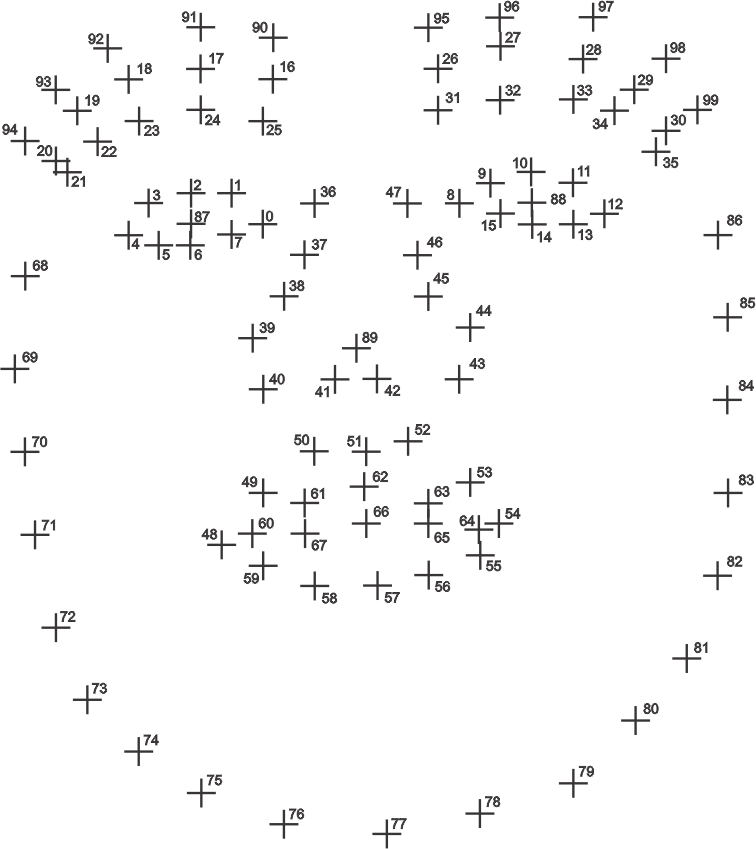
\includegraphics[width=0.6\textwidth]{images/view_points}}
	\caption{Representació dels punts de la cara que són utilitzats en la presa de dades}
\end{figure}

\section{Objectius}

L'objectiu d'aquest treball és poder decidir a partir d'una dada no usada prèviament:
\begin{enumerate}
	\item A partir d'una sola expressió facial si aquella s'està realitzant o no.
	\item A partir de tot el conjunt de dades si s'està realitzant o no una expressió facial.
	\item En el cas en el que s'estigui realitzant una expressió facial, poder decidir de quin tipus d'expressió facial (o paraula) es tracta.
	\item Trobar quin tipus de model s'adequa millor als objectius anteriors i comprar-los entre ells.
\end{enumerate}

\section{Procés d'exploració de dades}

S'han realitzat dos \emph{scripts} en R. El primer és per visualitzar les dades cronològicament (\verb|loadData.R|) i el segon és per poder interpretar-les a l'hora de realitzar una classificació (\verb|clustering.R|).

En aquest cas interessa més el segon ja que és el que tracta el problema de \emph{clustering}. S'han realitzat dos tipus d'algoritmes\cite{bishop} per projectar les dades, FDA i PCA. L'\emph{script} requereix que es seleccioni primerament quina expressió (\verb|*_datapoints.txt|) i a continuació quins resultats (\verb|*_targets.txt|) es volen agafar. També cal introduir de quin punt es volen visualitzar les dades (variable \verb|point|). 

A continuació es mostren els resultats obtinguts amb el conjunt de dades \verb|a_affirmative_datapoints.txt| i \verb|a_affirmative_targets.txt| i el punt 60 que correspon a la part superior del llavi. Per representar les dades s'han restat les mitjanes per tal que tant els punts com la recta de projecció estiguin centrades al voltant de $(0,0)$.

\begin{longtable}{cc}
	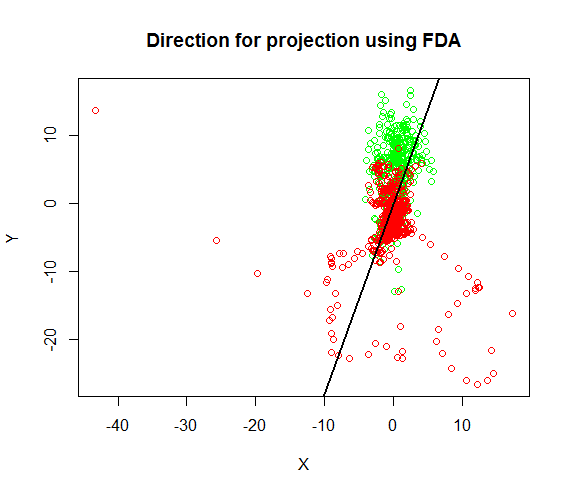
\includegraphics[width=0.45\textwidth]{images/FDA_XY} &
	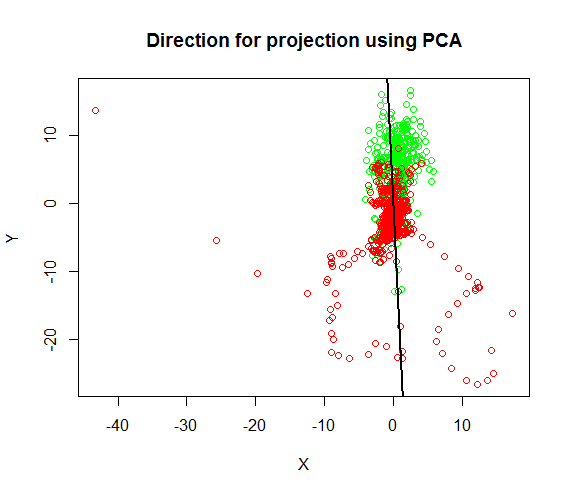
\includegraphics[width=0.45\textwidth]{images/PCA_XY} \\
	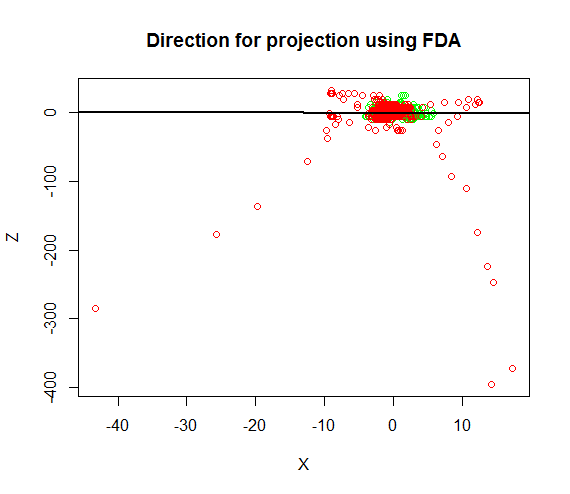
\includegraphics[width=0.45\textwidth]{images/FDA_XZ} &
	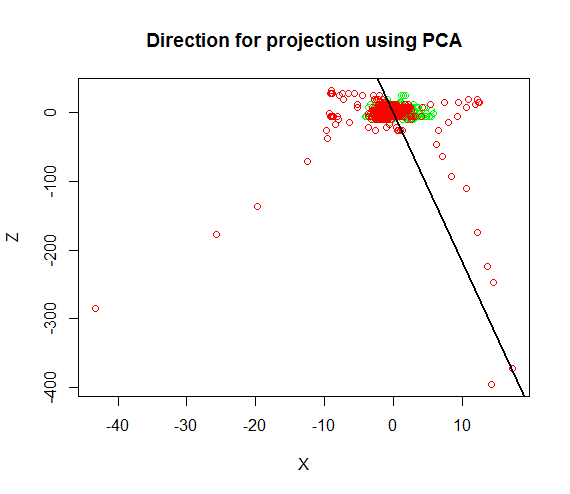
\includegraphics[width=0.45\textwidth]{images/PCA_XZ} \\
	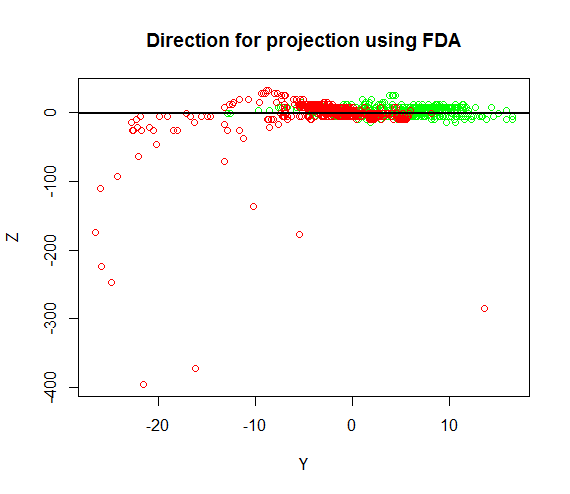
\includegraphics[width=0.45\textwidth]{images/FDA_YZ} &
	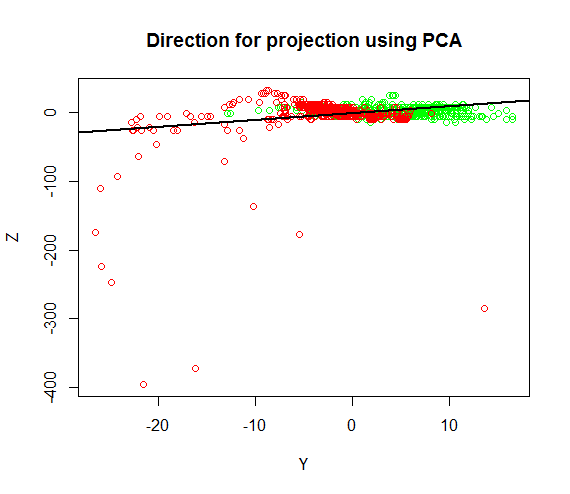
\includegraphics[width=0.45\textwidth]{images/PCA_YZ} \\
	\multicolumn{2}{c}{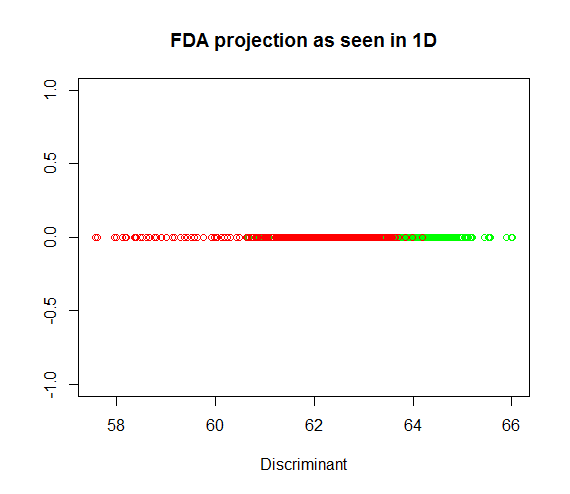
\includegraphics[width=0.5\textwidth]{images/FDA_projection}}
\end{longtable}

Com es pot veure als gràfics anteriors la dada Z no permet agrupar les dades gaire bé ja que totes queden al voltant dels valors \verb|Z = 0|. Tot i així es pot veure en les dimensions $X$ i $Y$ la separació de les dades es relativament fàcil. 

També, donat que sembla ser viable una projecció, es pot fer una projecció de cada punt de 3 dimensions a una sola dimensió.

\section{Resultats amb mètodes lineals/quadràtics}
Donat que hi ha diversos objectius en aquest treball s'han usat diferents mètodes per a poder resoldre cadascun dels objectius, han estat els següents:
\begin{itemize}
	\item Regressió logística i LDA:
	\begin{itemize}
		\item A partir d'una sola expressió facial si aquella s'està realitzant o no.
		\item A partir de tot el conjunt de dades si s'està realitzant o no una expressió facial.
	\end{itemize}
	\item MLP i LDA:
	\begin{itemize}
		\item En el cas en el que s'estigui realitzant una expressió facial, poder decidir de quin tipus d'expressió facial (o paraula) es tracta.
	\end{itemize}
\end{itemize}

\subsection{Detecció d'expressió facial amb regressió logística}
L'script \verb|logistic.R| realitza classificació amb regressió logística mitjançant l'ajuda de \verb|glm|. Per poder utilitzar l'script cal posar el \verb|Working Directory| a l'arrel de la carpeta subministrada i un cop es comença a executar cal escollir les dades que es volen usar per entrenar i les que es volen usar per validar.

En el primer experiment s'ha usat una sola expressió facial (dades contingudes a \verb|a_affirmative_datapoints.txt| i a \verb|a_affirmative_targets.txt|) com a entrenament i, tot seguit, s'han validat els resultats amb la mateixa expressió facial però realitzada per una altra persona (dades contingudes a \verb|b_affirmative_datapoints.txt| i a \verb|b_affirmative_targets.txt|). A la \autoref{tab:reglog_training1} i la \autoref{tab:reglog_training2} es poden veure els resultats obtinguts.

\begin{table}[H]
	\centering
	\def\arraystretch{1.5}
	\begin{tabular}{c|rr}
		& \multicolumn{2}{c}{Valor real} \\
		Valor predit & 0 & 1 \\
		\hline
		0 & 648 & 0 \\
		1 & 0 & 414 \\
	\end{tabular}
	\caption{Valors predits pel conjunt d'entrenament. L'error és d'un 0\%.}
	\label{tab:reglog_training1}
\end{table}

\begin{table}[H]
	\centering
	\def\arraystretch{1.5}
	\begin{tabular}{c|rr}
		& \multicolumn{2}{c}{Valor real} \\
		Valor predit & 0 & 1 \\
		\hline
		0 & 159 & 341 \\
		1 & 387 & 187 \\
	\end{tabular}
	\caption{Valors predits pel conjunt de validació. L'error és d'un 67,78\%.}
	\label{tab:reglog_training2}
\end{table}

En el segon experiment s'han usat totes les expressions facials d'una persona (dades contingudes a tots els arxius \verb|a_*.txt|) per a l'entrenament i per a la validació s'han usat totes les dades de l'altre persona (dades contingudes a tots els arxius \verb|b_*.txt|). Es poden veure els resultats a la \autoref{tab:reglog_training3} i la \autoref{tab:reglog_training4}.

\begin{table}[H]
	\centering
	\def\arraystretch{1.5}
	\begin{tabular}{c|rr}
		& \multicolumn{2}{c}{Valor real} \\
		Valor predit & 0 & 1 \\
		\hline
		0 & 8912 & 361 \\
		1 & 242 & 4095 \\
	\end{tabular}
	\caption{Valors predits pel conjunt d'entrenament. L'error és d'un 4,43\%.}
	\label{tab:reglog_training3}
\end{table}

\begin{table}[H]
	\centering
	\def\arraystretch{1.5}
	\begin{tabular}{c|rr}
		& \multicolumn{2}{c}{Valor real} \\
		Valor predit & 0 & 1 \\
		\hline
		0 & 5725 & 2962 \\
		1 & 3180 & 2459 \\
	\end{tabular}
	\caption{Valors predits pel conjunt de validació. L'error és d'un 42,87\%.}
	\label{tab:reglog_training4}
\end{table}

\subsection{Detecció d'expressió facial amb LDA}
L'script \verb|LDA_si_no.R| realitza classificació amb \emph{lda} mitjançant l'ajuda de \verb|lda|. Per poder utilitzar l'script cal posar el \verb|Working Directory| a l'arrel de la carpeta subministrada i un cop es comença a executar cal escollir les dades que es volen usar per entrenar i les que es volen usar per validar.

En el primer experiment s'ha usat una sola expressió facial (dades contingudes a \verb|a_affirmative_datapoints.txt| i a \verb|a_affirmative_targets.txt|) com a entrenament i, tot seguit, s'han validat els resultats amb la mateixa expressió facial però realitzada per una altra persona (dades contingudes a \verb|b_affirmative_datapoints.txt| i a \verb|b_affirmative_targets.txt|). A la \autoref{tab:lda_yes_no1} i la \autoref{tab:lda_yes_no2} es poden veure els resultats obtinguts.

\begin{table}[H]
	\centering
	\def\arraystretch{1.5}
	\begin{tabular}{c|rr}
		& \multicolumn{2}{c}{Valor real} \\
		Valor predit & 0 & 1 \\
		\hline
		0 & 626 & 72 \\
		1 & 22 & 342 \\
	\end{tabular}
	\caption{Valors predits pel conjunt d'entrenament. L'error és d'un 8,85\%.}
	\label{tab:lda_yes_no1}
\end{table}

\begin{table}[H]
	\centering
	\def\arraystretch{1.5}
	\begin{tabular}{c|rr}
		& \multicolumn{2}{c}{Valor real} \\
		Valor predit & 0 & 1 \\
		\hline
		0 & 182 & 267 \\
		1 & 364 & 261 \\
	\end{tabular}
	\caption{Valors predits pel conjunt de validació. L'error és d'un 58,75\%.}
	\label{tab:lda_yes_no2}
\end{table}

En el segon experiment s'han usat totes les expressions facials d'una persona (dades contingudes a tots els arxius \verb|a_*.txt|) per a l'entrenament i per a la validació s'han usat totes les dades de l'altre persona (dades contingudes a tots els arxius \verb|b_*.txt|). Es poden veure els resultats a la \autoref{tab:lda_yes_no3} i la 	\autoref{tab:lda_yes_no4}.

\begin{table}[H]
	\centering
	\def\arraystretch{1.5}
	\begin{tabular}{c|rr}
		& \multicolumn{2}{c}{Valor real} \\
		Valor predit & 0 & 1 \\
		\hline
		0 & 8876 & 459 \\
		1 & 278 & 3997 \\
	\end{tabular}
	\caption{Valors predits pel conjunt d'entrenament. L'error és d'un 5,42\%.}
	\label{tab:lda_yes_no3}
\end{table}

\begin{table}[H]
	\centering
	\def\arraystretch{1.5}
	\begin{tabular}{c|rr}
		& \multicolumn{2}{c}{Valor real} \\
		Valor predit & 0 & 1 \\
		\hline
		0 & 5018 & 2317 \\
		1 & 3887 & 3104 \\
	\end{tabular}
	\caption{Valors predits pel conjunt de validació. L'error és d'un 43,31\%.}
	\label{tab:lda_yes_no4}
\end{table}

\section{Resultats amb mètodes no lineals}
\section{Model final escollit}
\section{Conclusions}
\section{Possibles extensions}
\section{Referències}

\bibliographystyle{acm}
\bibliography{bibliography}

\end{document}